\renewcommand*\chapterpagestyle{scrheadings}
\chapter{Introduction}

This project aims to provide a voice assistant implementation that can be used with various frontends,
one such frontend being implemented parallel to this project using the Qt framework\footnote{Qt Framework \cite{qt}}.

\section{Project Scope}
The project scope encompassed the following objectives:
\begin{itemize}
    \item Efficient processing, with a target response latency of 1 second
    \item Integration into Linux windows managers, allowing users to operate their system using voice commands
    \item Functionality allowing explicit recording and voice activation
    \item Allowing the user to configure which algorithms or APIs they want to use, as well as the output format
\end{itemize}

\section{Background and Motivation}
Voice assistants have experienced steady adoption growth,
though they were often regarded as supplementary rather than essential tools.
This project sought to address this limitation
by developing a voice assistant frontend solution that could enhance users' workflows
while maintaining minimal intrusiveness.
The implementation focused on extending traditional voice assistant capabilities
with advanced features such as workspace management and speech-to-text integration.

\section{System Architecture}
\subsection{Technology Considerations}
Achieving low response latency is heavily influenced by the choice of the technology stack.
The initial prototype of the voice assistant was implemented using Kotlin and Spring Boot\footnote{Spring Framework \cite{spring}}, which offered flexibility and ease of development.
However, as the project evolved and introduced the stringent 1-second latency goal,
it became clear that a different approach was necessary.

To meet this performance requirement, a transition was made to Rust.
Rust was selected for its ability to produce highly optimized,
natively compiled binaries, making it ideal for applications requiring low latency.
Additionally, Rust's focus on memory safety and robust error handling
ensured the reliability of the application without compromising speed.
Previous experience with Rust further accelerated the development process,
making it the optimal choice for this project.

\subsection{Design}
The complete voice assistant consists of two parallel projects: this
Rust backend and a parallel Qt-frontend that is not part of the thesis.
The frontend serves as the user interface layer, providing efficient
access to the backend's voice processing capabilities.


The backend is designed with a modular architecture, enabling flexible configurations.
Each stage of the processing pipeline is
responsible for a specific aspect of the voice assistant's functionality,
allowing users to choose between a multitude of different processing methods,
whether local, remote, paid, or free.

The backend consists of the following stages:

\begin{itemize}
    \item \textbf{Recording Stage:} Implements both local and remote
    recording capabilities:
    \begin{itemize}
        \item Local Recorder for direct hardware access
        \item Remote Recorder for distributed setups
    \end{itemize}
    \item \textbf{Transcription Stage:} Provides multiple transcription
    options:
    \begin{itemize}
        \item Local Whisper for offline processing
        \item Cloudflare Whisper for edge computing
        \item OpenAI Whisper for cloud-based processing
    \end{itemize}
    \item \textbf{Processing Stage:} Implements various NLP options:
    \begin{itemize}
        \item Local NLP for offline processing
        \item Remote NLP for distributed processing
        \item Cloudflare NLP for edge computing
        \item OpenAI NLP for advanced language models
        \item Regex Matcher for simple pattern matching
    \end{itemize}
    \item \textbf{Output Stage:} Handles the final processing results
\end{itemize}

This modular approach ensures that the voice assistant can be tailored
to meet the specific needs and preferences of its users, providing a
robust and adaptable solution for voice interaction.

\begin{figure}[H]
    \centering
    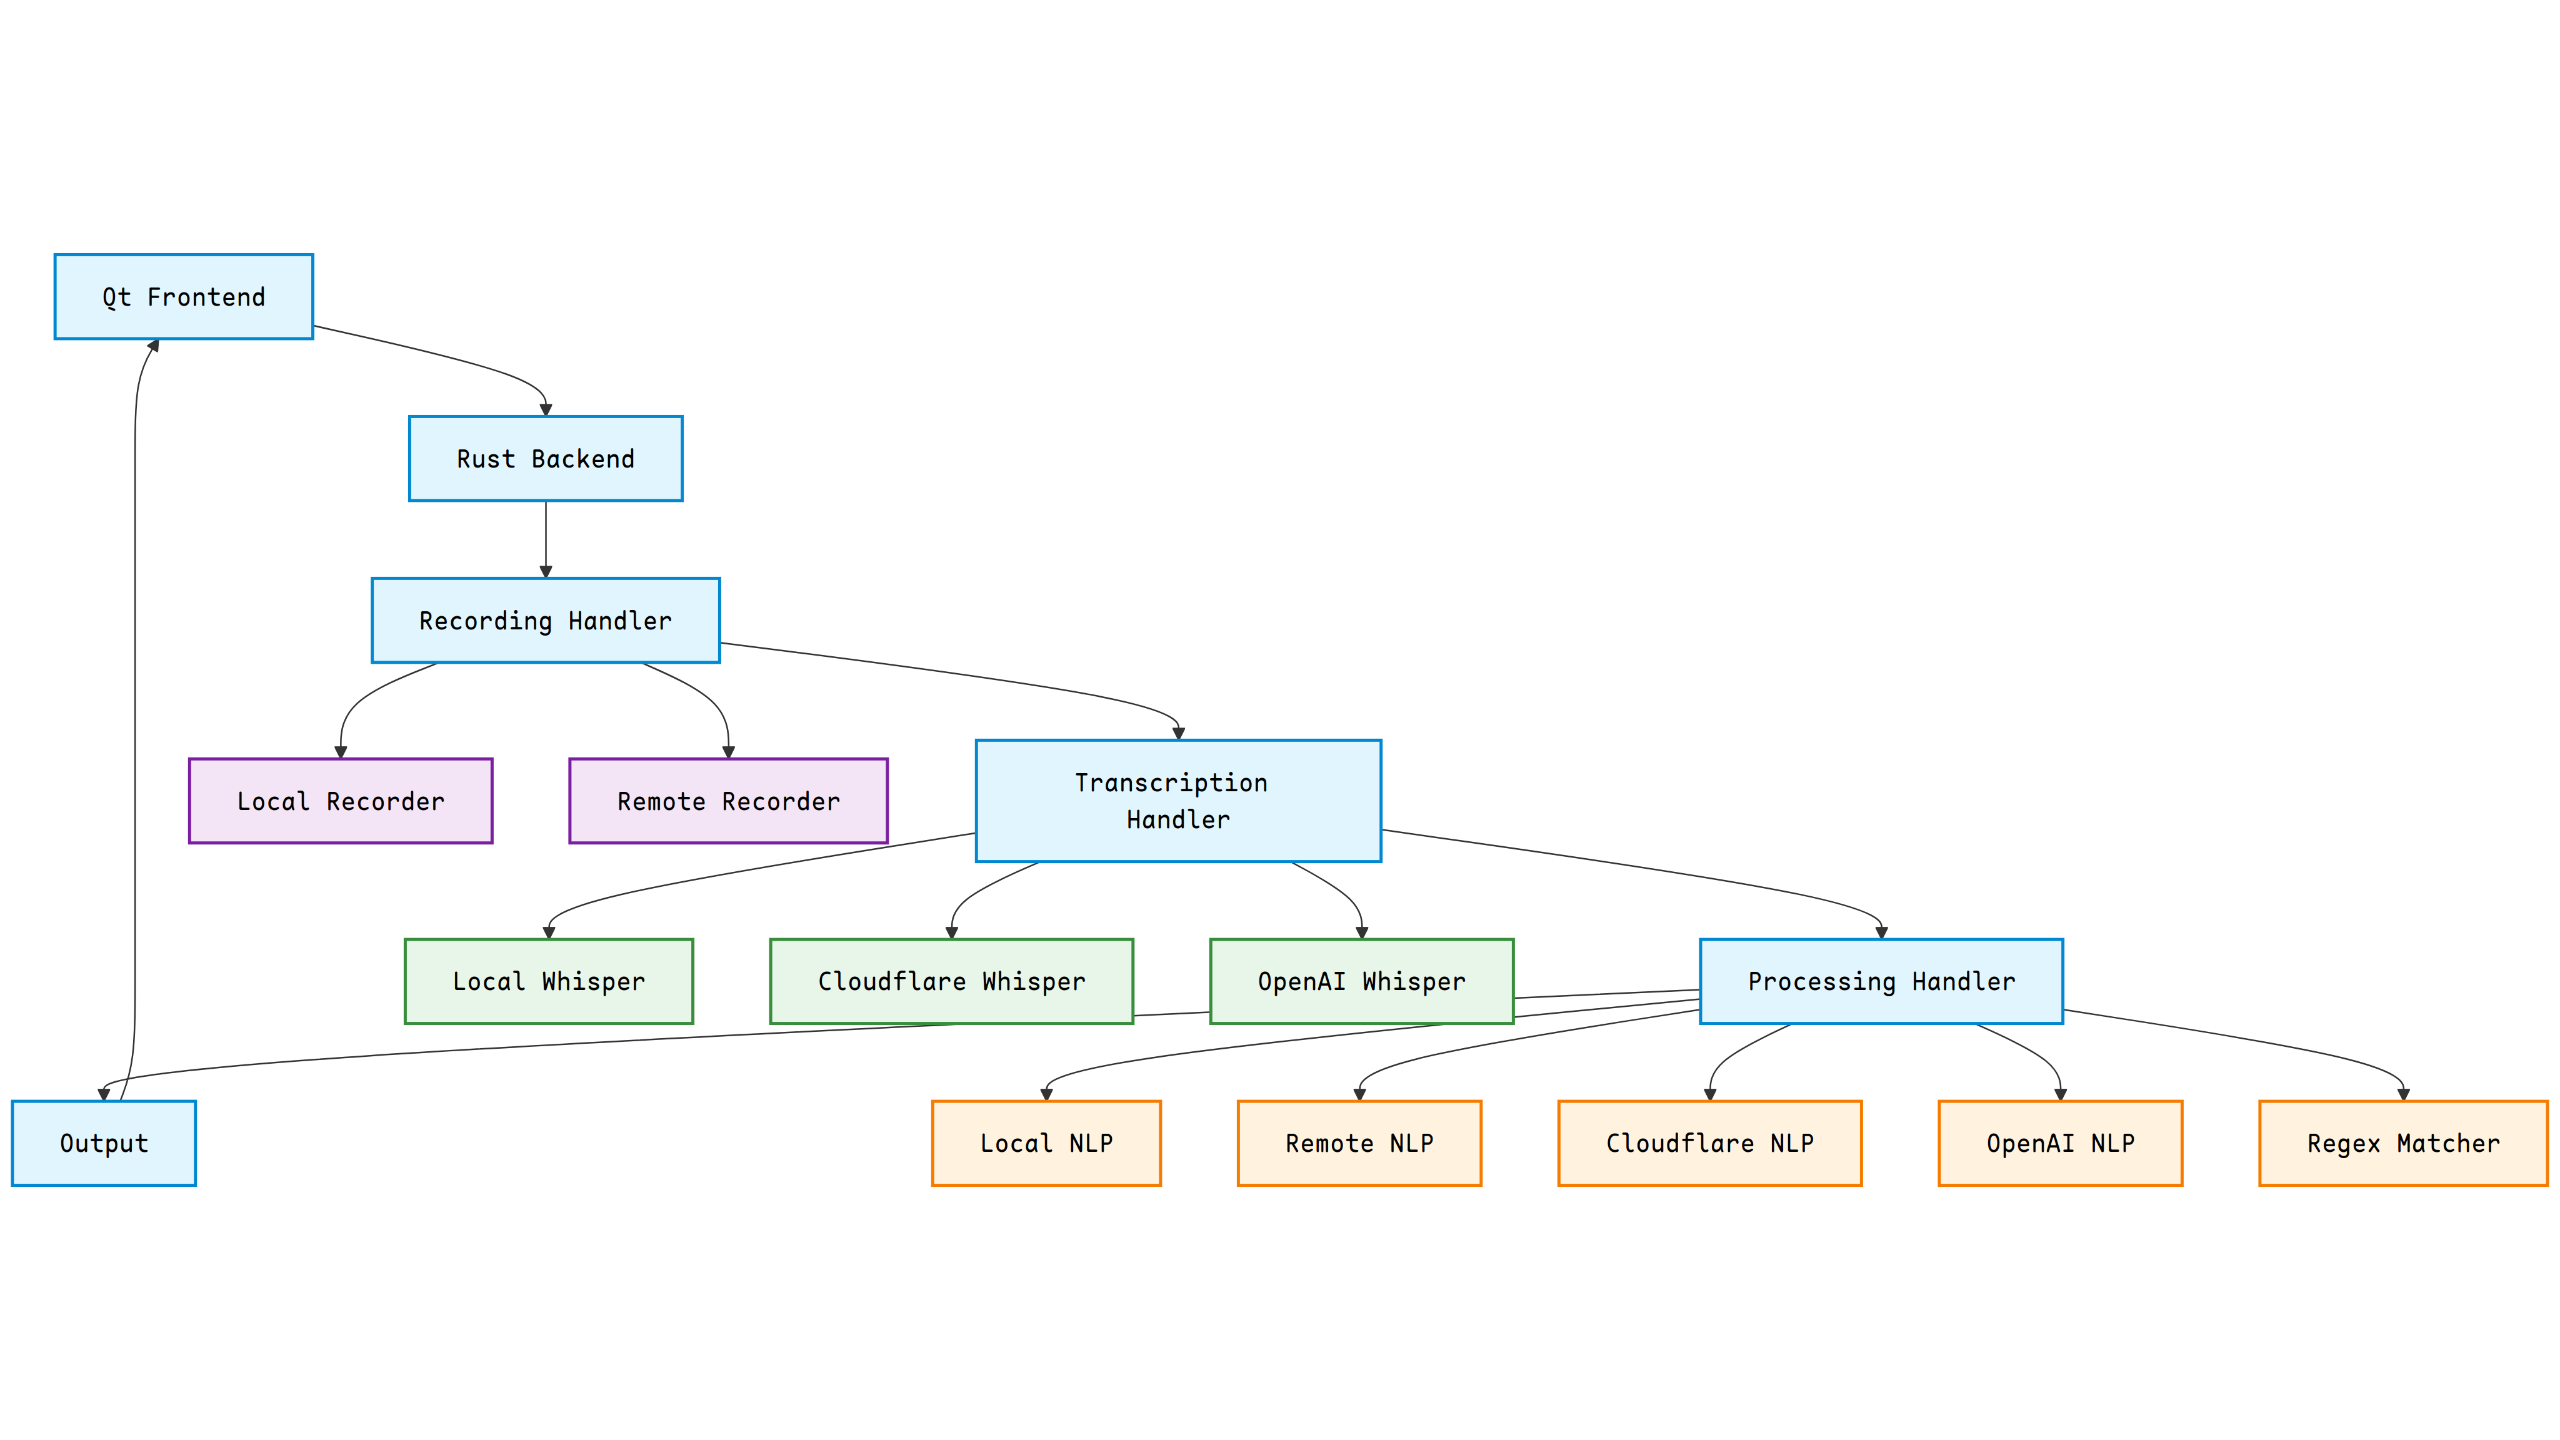
\includegraphics[width=\textwidth]{assets/stackchart}
    \caption{System architecture showing the Qt frontend (parallel
    running project) and the Rust backend components (this diploma
    thesis). The processing pipeline flows from the frontend through
    various backend stages, each offering multiple implementation
    options.}
    \label{fig:design}
\end{figure}